
https://www.smartdraw.com/uml-diagram/

https://www.planttext.com/?text=SoWkIImgAStDuU8gpixCKoZABqxbudBAJrBGjLDmpCbCJhLIy4ZDoSbNvE9oICrB0Qe40000
\begin{figure}
    \centering
    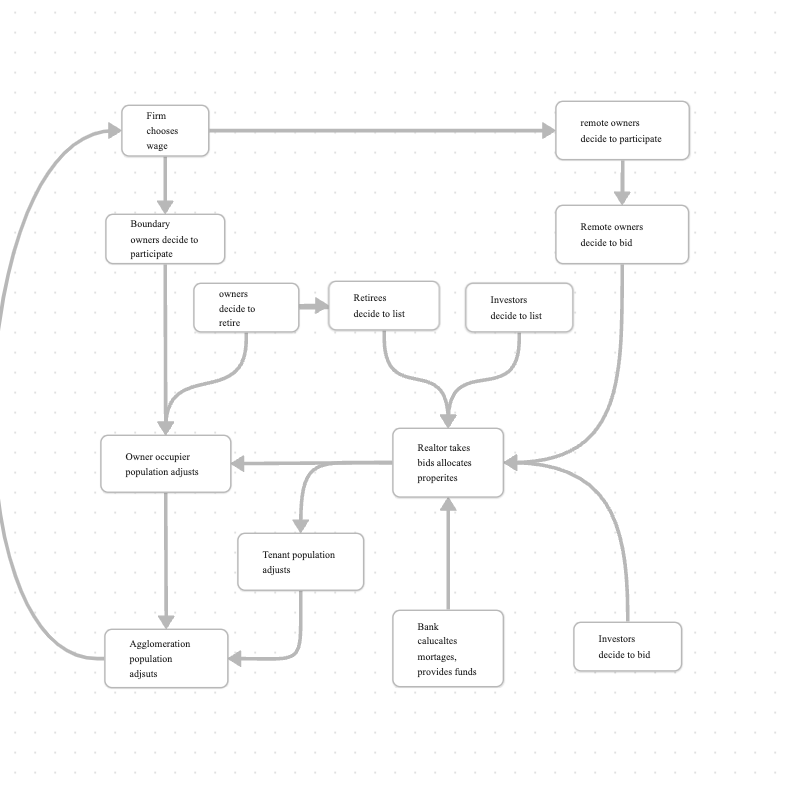
\includegraphics[width=0.5\linewidth]{informationflows.png}
    \caption{Enter Caption}
    \label{fig:enter-label}
\end{figure}

\https://us05web.zoom.us/j/89030886566?pwd=1CQlsuBMIbSlLPafb8nVH8pIDJFqbK.1

March 8: This is now in Chapter 11
The Transmission Puzzle, along with other revisions.
"we rewrite $A$ as
\[ A= A_0 + share * rent\]
$A_0$ represents outside capital, while $share*rent$ stands for the share of the urban locational rents captured by residents and  reinvested in productive capital. The share is composed of a propensity to invest locally and the actual land-ownership share of residents determined by the housing market. The investment might directly in production capital or indirectly through urban infrastructure such as transportation that cuts production costs.

More explicitly, for the code let sh stand for the owner-occupier share let Base_A = 3000
Let im Impoct share  be   = 1000
A = Base_A - (1-sh)* B_0 
i.e.
A = Base_A -B_0 + sh* B_0  

if effect_off:
    sh = 1.  A=
A = Base_A + sh * 1500
if its off then share is always - before investors buy in.. 
3500 100. ownership.. 


3500 will be same 

A is at o want it up. otherwise want it down.. 


This is the simplest possible model and centers the effect on the current model.



REVISE EQUITY BID I HAVE MADE THE NECESSARY CHANGES IN CHAPTER-MODEL LINE 444 FF and suggested correction in Agents line 368

We have line 336
 income_bid = 0.28 * (wage + r * S) / r_prime
You pointed out that  we can't get interest on savings we buy a house with , which is (1-m)*income_bid = M. 

Therefore we should have

income_bid = 0.28 * (wage + r * (S-(1-m)*income_bid)) / r_prime
           = 0.28 * (wage + r * (S)) / r_prime
            - 0.28 * (1-m)*income_bid) / r_prime
income_bid*(1+0.28 * (1-m)*income_bid) / r_prime) 
                    =0.28 * (wage + r * (S)) / r_prime
 income_bid         =  (0.28 * (wage + r * (S)) / r_prime)   /(1+0.28 * (1-m)*income_bid)/ r_prime 

 income_bid = (0.28 * (wage + r * (S))  /(r_prime + 0.28 * (1-m)*income_bid)



base) davidroomputer3:housing_app drdavidrobinson$ python run.py
Fast batch
Traceback (most recent call last):
  File "run.py", line 156, in <module>
    df, variable_parameters = fast_batch()
  File "run.py", line 94, in fast_batch
    from model.model_fast import Fast
  File "/Users/drdavidrobinson/Devel/housing_app/model/model_fast.py", line 11, in <module>
    from model.time import RandomActivationByType
  File "/Users/drdavidrobinson/Devel/housing_app/model/time.py", line 26
    from __future__ import annotations
    ^
SyntaxError: future feature annotations is not defined
(base) davidroomputer3:housing_app drdavidrobinson$
 ############   MODEL 1  --- MARCH 1   ############ 
        # self.model.model_description = "March 2 ensure we still have the model working"
    
        # self.k_target = self.price_of_output * self.alpha * self.y/self.r     #(old optimal version)
        # self.n_target   = 5 * (self.beta* self.A * self.agglom_pop**self.gamma *  self.k**self.alpha )**(1-self.beta) 
        # self.worker_demand = self.n_target * self.F # self.n_target * self.F_target
        # edr = (self.worker_demand - self.worker_supply) / max(abs(self.worker_demand), abs(self.worker_supply)) #positive or negative 
        # self.F = self.worker_supply / self.n  #moved this up two lines
        # self.wage_target =  VMPL / ov
        # self.wage        = self.wage_target  #(1 - self.adjw) * self.wage_target + self.adjw * self.wage_target
        
        # #INCREMENT STATE VARIABLES TOWARDS TARGETS
        # self.n        = (1 - self.adjn) * self.n + self.adjn * self.n_target
        # self.k        = (1 - self.adjk) * self.k + self.adjk * self.k_target 
        # # self.F      = (1 - self.adjF) * self.F + self.adjF * self.F_target
        # self.wage     = (1 - self.adjw) * self.wage + self.adjw * self.wage_target  #reintroduced  - didn't help
        # #self.y       = (1 - self.adjy) * self.y + self.adjy * self.y*F_target 

        # self.wage_premium     = self.wage - self.subsistence_wage # find wage available for transportation
        # self.p_dot            = self.get_p_dot()
        # # COMMENT: wage goes to 100,000 with 5 in n_target  Mult=1, but n=12
      
     ############   MODEL 2  --- MARCH 3   ############ 
        self.model.model_description = "March 3 den increases firms nothing else "
        self.k_target = self.price_of_output * self.alpha * self.y/self.r     #(old optimal version)
        self.n_target   = 5 * (self.beta* self.A * self.agglom_pop**self.gamma *  self.k**self.alpha )**(1-self.beta) 
        self.worker_demand = self.n_target * self.F # self.n_target * self.F_target
        edr = (self.worker_demand - self.worker_supply) / max(abs(self.worker_demand), abs(self.worker_supply)) #positive or negative 
        self.F = self.worker_supply / self.n  #moved this up two lines
        self.wage_target = (1 + edr) * VMPL / ov  # this is the innovationn in this veersion March 3
        self.wage        = self.wage_target  #(1 - self.adjw) * self.wage_target + self.adjw * self.wage_target
        
        # INCREMENT STATE VARIABLES TOWARDS TARGETS 
        self.n        = (1 - self.adjn) * self.n + self.adjn * self.n_target
        self.k        = (1 - self.adjk) * self.k + self.adjk * self.k_target 
        # self.F        = (1 - self.adjF) * self.F + self.adjF * self.F_target
        self.wage     = (1 - self.adjw) * self.wage + self.adjw * self.wage_target  #reintroduced  - didn't help
        #self.y        = (1 - self.adjy) * self.y + self.adjy * self.y*F_target 

        self.wage_premium     = self.wage - self.subsistence_wage # find wage available for transportation
        self.p_dot            = self.get_p_dot()
        # COMMENT: mult=1 1-> 1.2 no dif? density increases F, beta[0.73, .78]increases wneFN low alpha very inhibiting
        # COMMENT:adjN no effect if adj k high, overshoot adjn no effect


     ############   MODEL 3  --- MARCH UNCHANGED    ############ 
        #  self.model.model_description = "March 2 ensure we still have the modle working"        self.k_target = self.price_of_output * self.alpha * self.y/self.r     #(old optimal version)
        # self.n_target   = 1 * (self.beta* self.A * self.agglom_pop**self.gamma *  self.k**self.alpha )**(1-self.beta) 
        # self.worker_demand = self.n_target * self.F # self.n_target * self.F_target
        # edr = (self.worker_demand - self.worker_supply) / max(abs(self.worker_demand), abs(self.worker_supply)) #positive or negative 
        # self.F = self.worker_supply / self.n  #moved this up two lines
        # self.wage_target =  VMPL / ov
        # self.wage        = self.wage_target  #(1 - self.adjw) * self.wage_target + self.adjw * self.wage_target
        
        # #TODO INCREMENT STATE VARIABLES TOWARDS TARGETS     NOT USED  REMOVE?
        # self.n        = (1 - self.adjn) * self.n + self.adjn * self.n_target
        # self.k        = (1 - self.adjk) * self.k + self.adjk * self.k_target 
        # # self.F        = (1 - self.adjF) * self.F + self.adjF * self.F_target
        # self.wage     = (1 - self.adjw) * self.wage + self.adjw * self.wage_target  #reintroduced  - didn't help
        # #self.y        = (1 - self.adjy) * self.y + self.adjy * self.y*F_target 

        # self.wage_premium     = self.wage - self.subsistence_wage # find wage available for transportation
        # self.p_dot            = self.get_p_dot()

    
- Do tenants get ripped off more than owners?


K's questions

1. Go over when investors list homes for sale, because currently they never sell in the main code
2. Talk through  how we will track mortgage share - e.g. how much do people - borrow most they can to purchase the house. but how much do they pay down?
Do we initialize the city with any kind of moortgages, so we want it as a share of sold houses.b


    
Other questions
- What measures do we use for location of rentors/location of investors? 
  - (share by distance from center plotted as line?) -- total share of boundary as a function of time (rent to be captured is larger near the center)
  - Also want to see - share of houses that have been sold as a function of distance... 



   
%%%%%%%%%

For amenity. Add a value of A_j for each property. We assume A is in dollars and put it into person_bid price by adding it to property valuation.

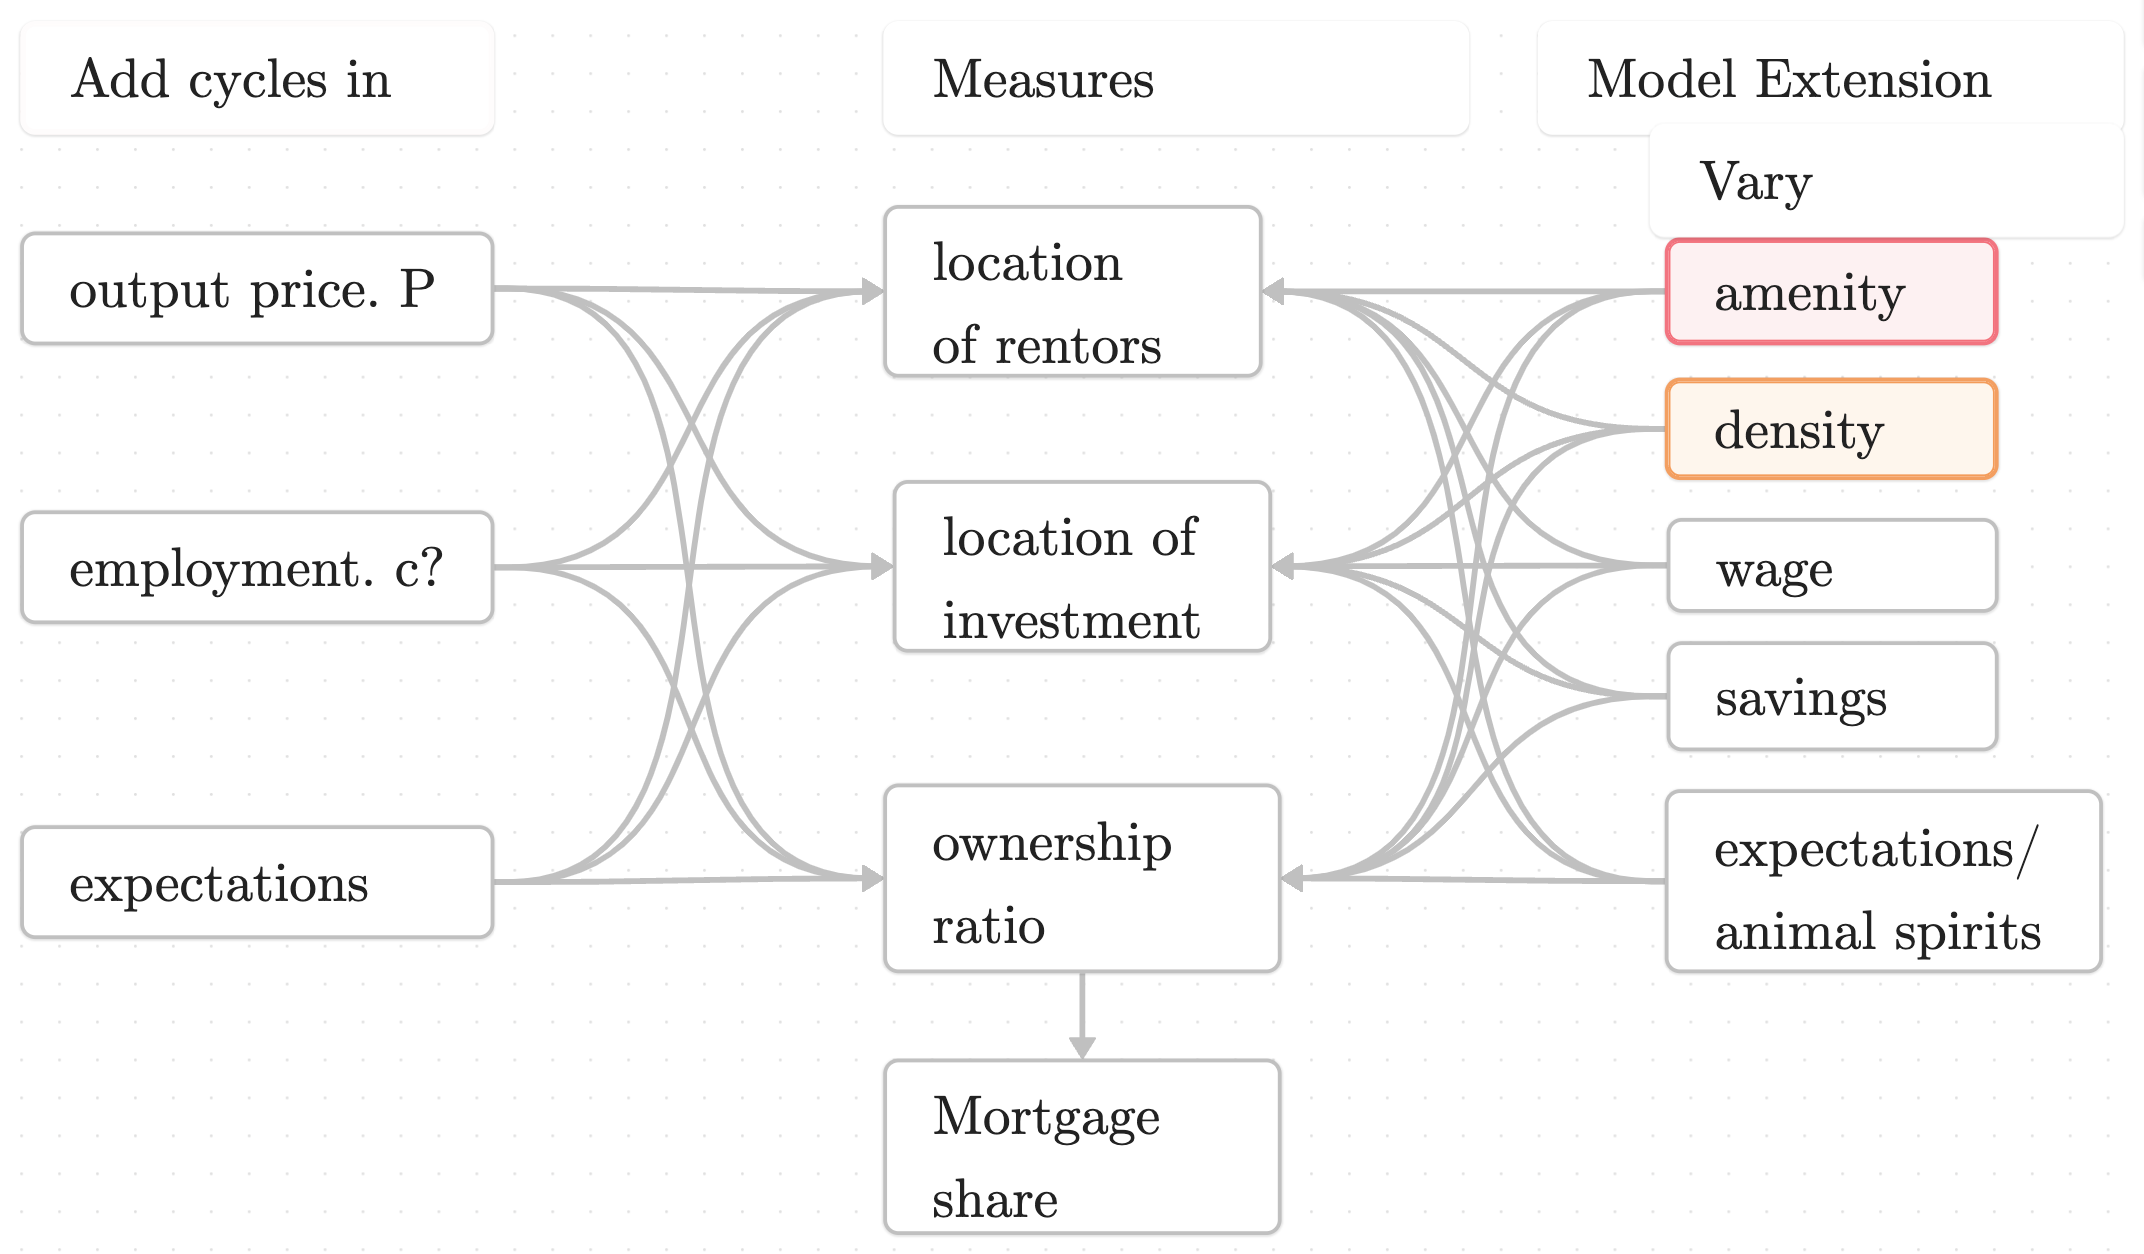
\includegraphics[]{/fig/models_and_measures}

To get individual preferences, add a value to each person A taste parameter 0<T_i < 4. Then, in calculating the value of the property use    T_i*A_j

Add a density to each location. (does density then go into bid price for speculators?) 

Add a wage differential factor 0< wdf_i < 4 to each person. Their income is then wage*wdf_i


Does this work?  Define self.bank.expectations_shock  as a time varying scalar centred on 1.0

    def get_max_desired_bid(self, R_N, r, r_target, m, p_dot, capital_gains_tax, transport_cost, expectations_shock):
        T      = self.model.mortgage_period
        delta  = self.model.delta
        # capital_gains_tax = self.model.capital_gains_tax # person and investor send.

        if R_N is not None and r is not None and r_target is not None and m is not None and p_dot is not None:
            R_NT   = ((1 + r)**T - 1) / r * R_N
            # return R_NT / ((1 - m) * r_target/(delta**T) - p_dot) 
            return (1 - capital_gains_tax) * R_NT / ((1 - m) * r_target/(delta**T) - self.bank.expectations_shock * p_dot +(1+r)**T*m) # Revised denominator from eqn 6:20

        else:
            self.model.logger.error(f'Get_max_desired_bid None error Rn {R_N}, r {r}, r_target {r_target}, m {m}, p_dot {p_dot}', expectations_shock
)
            return 0. # TODO Temp


Traditional sampling techniques (grid vs random vs sobol vs latin hypercube)
https://www.youtube.com/watch?app=desktop&v=Evua529dAgc


https://salib.readthedocs.io/en/latest/

https://doepy.readthedocs.io/en/latest/#:~:text=At%20its%20heart%2C%20doepy%20is,arbitrary%20range%20of%20input%20variables.




## Hypotheses
The financial sector affects the ownership of housing and the class structure of society, 
There may be dynamic/resilience features of this model that make the effects worse than you might expect
- Boom bust - pump wealth on/out of city on the boom and on the bust. 'There are sharks in the water' 1. Higher bid can amplify up swings - have to compete with speculators 2. can't get it back on down swing since outside finance offers a stable floor- buys up on way down (we expect larger effects as people are 1. displaced on the way up and then 2. evicted on the way down - can't use their spaces)
  - reduce demand for labour temporarily - reduce wages for labour - demand -- cyclic structure - local employment structure - and financial booms that are external.. - cases where they align and where they do not
  - link finance and employment -vary price of output- vary the employment *** 
- Hysteresis - perturb, doesn't come back - e.g. interest rates go up.
- The way it aligns with long run changes in the landscape e.g. tech changing local info changes vulnerability to these shocks -- Depth of the basin changes - er   odes systemic resilience - together these changes bo the capacity to hold value in landscape. (links to the productivity feedback - much will/can they invest in increasing their productivity/supporting kids/good food to grow brains. Education to increase productivity is the feature that makes productivity increases resilient to de-industrialization)
This has implications for landscape- system- class structure- 

This may have implications for urban productivity. (can actually displace productive uses - empty store fronts) - who can/will enter, how , who can rent spaces, speculative value may keep it empty (work spaces or living space - lowering pop), reduces consumption


Amplified effects by extensions
Two city experiments
Different incomes  - inequality
Urban density



## High Priority
imediately do experiments with the price of output - should give a decline in price of labour, may or may not result in changes in the housing market (record housing prices]
Which interest rate is charged to investors
speed/memory, plot and workflow to find parameters, run online - try storing the bid rent curve -- - what is the gap.. 

just keep housing - turn off storage..  cyclic pieces turn off the market. - turn off the production







source activate housing
conda install -c conda-forge mesa
avid-robinsons-computer-3:housing_app drdavidrobinson$ conda env create -f environment.yml -n housing
Collecting package metadata (repodata.json): done
Solving environment: failed

            does investor share begin to rise (defined as ``for a given number of steps - say 70 - where is $Z=share_t - share_{t-1} \ge 0$? ) and where does it fall.

Maybe just store Z and and draw contour lines - there has to be as program for that.


